\documentclass[10pt]{article}

\usepackage[USenglish,spanish,es-tabla]{babel}
\usepackage[utf8]{inputenc}
\usepackage{authblk}
\usepackage{csquotes}
\usepackage{lipsum}
\usepackage{amsmath}
\usepackage{amssymb}
\usepackage{gensymb}
\usepackage{textcomp}
\usepackage{enumerate}
\usepackage{enumitem}
\usepackage{bm}
\usepackage{nicefrac}
\usepackage{abstract}
\usepackage{titlesec}
\usepackage{microtype}
\usepackage[margin=2cm]{geometry}
\usepackage{pdfpages}
\usepackage{graphicx}
\usepackage[centerlast]{subfigure}
\usepackage{float}
\usepackage{booktabs}
\usepackage{multicol}
\setlength{\columnsep}{0.75cm}
\spanishdecimal{.}	
\usepackage[justification=centerlast]{caption}
\usepackage{hyperref}
\hypersetup{
    colorlinks=true,
    linkcolor=black,
    filecolor=black,      
    urlcolor=blue,
    citecolor=black,
}
\urlstyle{same}

%\titleformat{\section}
%{\centering\normalfont\bfseries}
%{\thesection.}{0.25cm}{}
%\renewcommand{\thesection}{\Roman{section}}
%
%
%\titleformat{\subsection}
%{\centering\normalfont\scshape}
%{\thesubsection.}{0.25cm}{}
%\renewcommand{\thesubsection}{\thesection.\Roman{subsection}}
%
%\titleformat{\subsubsection}
%{\centering\normalfont\scshape}
%{\thesubsubsection.}{0.25cm}{}
%\renewcommand{\thesubsubsection}{\thesubsection.\Roman{subsubsection}}

%\usepackage[backend=bibtex, bibencoding=ascii,sorting=none]{bibtex}
%\addbibresource{bib.bib}


\usepackage{titling}
\setlength{\droptitle}{-1.5cm}

\setlength\parindent{0pt}

\usepackage{xcolor}

%\pagecolor[rgb]{0,0,0}
%\color[rgb]{1,1,1}

\title{\textbf{Ataque adversarios} \vspace{-0.25em}} 
\author{Enrique David Guzmán Ramírez \vspace{-1em}}
\affil{IIMAS, Universidad Nacional Autónoma de México \vspace{-0.5em}}
\affil{Introducción al Aprendizaje Profundo \vspace{-0.25em} \\  M. en C. Berenice Montalvo Lezama \\ M. en C. Ricardo Montalvo Lezama}

\renewcommand\Affilfont{\normalsize}

\date{{\normalsize \today}}

\begin{document}	

\maketitle

\begin{abstract}
Las redes neuronales profundas son modelos poderosos que se han utilizado ampliamente para lograr un rendimiento cercano al nivel humano en una variedad de tareas. Sin embargo, a pesar de su desempeño superior estudios recientes han encontrado que incluso los modelos del estado del arte son sumamente vulnerables a ataques adversarios. En el presente trabajo se exploran algunos de los algoritmos de ataques adversarios en algunas de las arquitecturas más recientes de visión computacional.
\end{abstract}

\begin{multicols*}{2}

\section{Introducción}

Un ataque adversario es una muestra de datos de entrada que ha sido perturbada
levemente con la intención de hacer fallar a un clasificador

En muchos casos, estas modificaciones pueden ser tan sutiles que un observador humano ni siquiera nota la modificación, pero el clasificador comete un error. Los ejemplos de adversarios plantean problemas de seguridad porque podrían usarse para realizar un ataque a los sistemas de aprendizaje automático, incluso si el atacante no tiene acceso al modelo subyacente.

Con la introducción de modelos de aprendizaje profundo en cada vez más distintos aspectos de nuestra vida, los problemas que estos ataques adversarios pueden ocasionar
son preocupantes.

\begin{figure}[H]
\centering
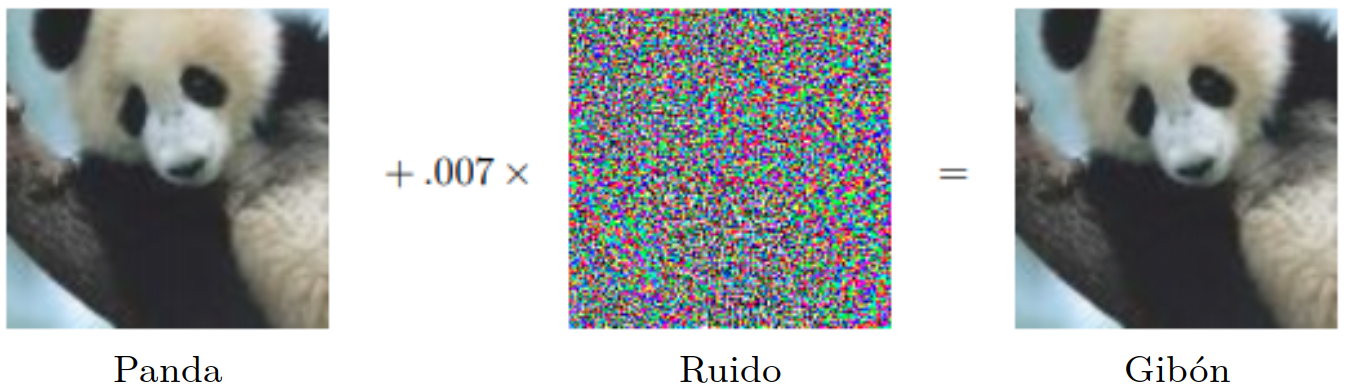
\includegraphics[width=0.99\linewidth]{Images/ejemplo1_anotado.png}
\caption{Ejemplo de ataque adversario. Imagen tomada de \href{https://arxiv.org/pdf/1412.6572.pdf}{\emph{Explaining and harnessing adversarial examples}.}}
\end{figure}

Los escenarios de posibles ataques adversarios se pueden clasificar en diferentes maneras:

\begin{itemize}
\item \textbf{Ataque no dirigido:} el objetivo es hacer que el clasificador prediga una etiqueta incorrecta, la etiqueta incorrecta específica no importa.

\item \textbf{Ataque dirigido:} el objetivo es cambiar la predicción del clasificador a alguna clase objetivo específica.
\end{itemize}

En segundo lugar, los escenarios de ataque se pueden clasificar por la cantidad de conocimiento que el adversario tiene sobre el modelo:

\begin{itemize}
\item \textbf{Caja negra:} el atacante no sabe mucho sobre el modelo, pero puede sondear o consultar el modelo, es decir, darle algunas entradas y observar salidas.

\item \textbf{Caja blanca:} el atacante tiene pleno conocimiento del modelo, como la arquitectura del modelo y los valores de todos los parámetros y pesos entrenables.
\end{itemize}

\subsection{Algoritmos de ataques adversarios}

Hay una multitud \cite{OnePixel}

\section{Objetivo}

El objetivo del proyecto es explorar y desarrollar algunas de las técnicas usadas para generar ataques adversarios así como explorar algunos de los métodos de defensa que existen.

\bibliographystyle{ieeetr}
\bibliography{bib.bib}

\end{multicols*}

\end{document}
